% Provenance (never printed): see sources/outline_sources.md (Year 2: humidity variables;
% Clausius--Clapeyron applied; dry and moist adiabats; thermodynamic diagrams; convective
% instability; cloud microphysics). Definitions after the NWS glossary; skew-T lines, CAPE classes
% and the lifted index after the NWS Houston/Galveston training page; saturation data from the
% NIST WebBook (IAPWS-95) and IAPWS R14-08; the empirical formula as used by Su and others
% (2026); kappa-Koehler theory after Petters and Kreidenweis (2007); CCN numbers after Andreae
% (2009); the processes of microphysics after Morrison and others (2020). The sounding is the
% real 12 UTC sounding of Norman, Oklahoma, 16 April 2026 (IGRA2); every curve and number from
% figdata/bachelor-2/thermo.py; exercise and problem values in the Book 4 scratch calculator
% calc/ch21.py.
\chapter{Thermodynamica van de atmosfeer}\label{ch:b2:atmospheric-thermodynamics}

Op 16 april 2026, om 12 UTC, steeg een ballon op van het weerstation van Norman, Oklahoma, zoals
er elke dag op dat uur ballonnen opstijgen van meer dan achthonderd stations. Het instrument dat hij
droeg, zond een verticaal profiel terug dat een weervoorspeller in één oogopslag leest: lucht bij de grond
bijna verzadigd, een dun warm deksel op zeshonderd meter hoogte, en daarboven een temperatuur die
tien kilometer lang snel daalde. Door het deksel opgetild, zou de oppervlaktelucht zich
over het grootste deel van de troposfeer warmer dan haar omgeving hebben bevonden, met zo'n tweeduizend joule per
kilogram om aan stijgen te besteden. Dit hoofdstuk leert die energie uit een sondering af te lezen: hoeveel
water lucht bevat, hoe een stijgend pakketje afkoelt vóór en na condensatie, hoe de diagrammen van
meteorologen oppervlakten in energieën omzetten, en hoe wolkendruppels überhaupt ontstaan.
% ledger: data:b4-sounding, nws4:upperair, nws4:cape

\begin{recall}
\textbf{Uit de natuurkundeboeken}: verzadigingsdampdruk, relatieve vochtigheid, dauwpunt,
latente warmte, de betrekking van Clausius--Clapeyron en haar geïntegreerde vorm; nucleatie en
onderkoeling; de eerste hoofdwet, adiabatische veranderingen en de warmtecapaciteiten van een ideaal gas.
\textbf{Uit de scheikundeboeken}: partiële drukken, de wet van Raoult, oppervlaktespanning en de
kelvinvergelijking. \textbf{Uit de schoolboeken}: het \omterm{def:b2:atmospheric-thermodynamics:lcl}{condensatieniveau} en zijn regel van
\qty{125}{m} per graad, stabiele en onstabiele lucht, de \omterm{def:b2:atmospheric-thermodynamics:microphysics}{condensatiekern}, het warmeregenproces en het
ijskristalproces. \textbf{Uit Boek~3}: de standaardatmosfeer, de omgevingsgradiënt
en de droogadiabatische gradiënt ($\Gamma_d = \qty{9.8}{K/km}$), het luchtpakketje, de potentiële
temperatuur, statische stabiliteit, temperatuurinversies en de hypsometrische vergelijking.
\end{recall}

In het hele hoofdstuk: $R_d = R/M_d = \qty{287.0}{J.kg^{-1}.K^{-1}}$ voor droge lucht met molaire massa
\qty{28.97}{g/mol}; $R_v = R/M_w = \qty{461.5}{J.kg^{-1}.K^{-1}}$ voor waterdamp, met molaire
massa \qty{18.0153}{g/mol}; $\varepsilon = M_w/M_d = 0.622$; $c_p = \tfrac72 R_d =
\qty{1004.5}{J.kg^{-1}.K^{-1}}$ (Boek~3, met de verhouding van de warmtecapaciteiten 1.4);
$g = \qty{9.81}{m.s^{-2}}$; en de verdampingswarmte bij het tripelpunt,
$L = \qty{2.501e6}{J/kg}$.
% ledger: const:R, earth:Mmol, nist4:water-mw, nasa:grc-gamma, const:gn, nist4:water-sat

\section{Vochtige lucht}\label{sec:b2:atmospheric-thermodynamics:moist-air}

Lucht is een mengsel van droge lucht en waterdamp, beide bijna ideale gassen. De natuurkundeboeken
meten haar water met de relatieve vochtigheid en het dauwpunt; een stijgend pakketje heeft maten nodig
die niet veranderen wanneer het uitzet.

\begin{definition}[Dampdruk; mengverhouding; specifieke vochtigheid]\label{def:b2:atmospheric-thermodynamics:moist-air}
De \emph{dampdruk}\index{dampdruk} $e$ van vochtige lucht is de partiële druk van
haar waterdamp. Haar \emph{mengverhouding}\index{mengverhouding} is $r = m_v/m_d$, de massa
waterdamp per massa-eenheid droge lucht in hetzelfde volume, en haar \emph{specifieke
vochtigheid}\index{specifieke vochtigheid} is $q = m_v/(m_d + m_v)$, de massa damp per massa-eenheid
vochtige lucht. Beide worden meestal in gram per kilogram gegeven.
\end{definition}
% ledger: nws4:humidity

\begin{proposition}[Vochtigheidsgrootheden]\label{prop:b2:atmospheric-thermodynamics:humidity}
In vochtige lucht bij de totale druk $p$ met de \omterm{def:b2:atmospheric-thermodynamics:moist-air}{dampdruk} $e$ geldt
\[
  r = \frac{\varepsilon e}{p - e}, \qquad q = \frac{r}{1 + r} = \frac{\varepsilon e}{p - (1 -
  \varepsilon)e} .
\]
Bij verzadiging is $e = e_s(T)$ en $r = r_s(T, p)$, de verzadigingsmengverhouding. Noch $r$ noch
$q$ verandert wanneer een pakketje uitzet of wordt samengedrukt zonder water op te nemen of te verliezen.
\end{proposition}

\begin{proof}
In hetzelfde volume $V$ bij de temperatuur $T$ gehoorzaamt elk gas aan zijn eigen idealegaswet met zijn
partiële druk: $m_v = eV/(R_vT)$ en $m_d = (p - e)V/(R_dT)$, dus $r = (R_d/R_v)\,e/(p - e)$,
en $R_d/R_v = M_w/M_d = \varepsilon$. Deling van $m_v$ door $m_d + m_v$ geeft $q = r/(1 + r)$.
Uitzetting verandert $V$, $p$ en $e$, maar niet de twee massa's.
\end{proof}

\begin{definition}[Virtuele temperatuur]\label{def:b2:atmospheric-thermodynamics:virtual}
De \emph{virtuele temperatuur}\index{virtuele temperatuur} $T_v$ van vochtige lucht is de temperatuur
die droge lucht bij dezelfde druk nodig zou hebben om dezelfde dichtheid te hebben:
\[
  T_v = T\,\frac{1 + r/\varepsilon}{1 + r} \approx T\,(1 + 0.61\,r) .
\]
\end{definition}
% ledger: nws4:virtual-theta-e

Het bewijs dat deze temperatuur doet wat ze belooft, is één regel: de dichtheid van vochtige lucht is
$(m_d + m_v)/V = \bigl(p - e\bigr)/(R_dT) + e/(R_vT)$, wat met $e = pr/(\varepsilon + r)$
gelijk is aan $p/(R_dT_v)$. Waterdamp is lichter dan droge lucht, dus vochtige lucht is minder dicht dan droge
lucht bij dezelfde temperatuur en druk, alsof ze een beetje warmer was.

\begin{example}[De lucht in Norman]\label{ex:b2:atmospheric-thermodynamics:norman}
Aan de grond geeft de sondering $p = \qty{971.1}{hPa}$, $T = \qty{19.0}{\celsius}$ en een dauwpunt
van \qty{18.5}{\celsius}. De \omterm{def:b2:atmospheric-thermodynamics:moist-air}{dampdruk} is de verzadigingsdampdruk bij het
dauwpunt, $e = e_s(\qty{18.5}{\celsius}) = \qty{21.5}{hPa}$ (\cref{prop:b2:atmospheric-thermodynamics:es}
verderop). Dan is $r = 0.622 \times 21.5/(971.1 - 21.5) = \qty{14.1}{g/kg}$, $q = \qty{13.9}{g/kg}$,
en $T_v - T = 0.61 \times 0.0141 \times \qty{292.15}{K} = \qty{2.5}{K}$: deze lucht is zo licht als
droge lucht die tweeënhalve graad warmer is.
\end{example}
% ledger: data:b4-sounding

\section{Verzadigingsdampdruk}\label{sec:b2:atmospheric-thermodynamics:saturation}

Boven een vlak oppervlak van zuiver water hangt de \omterm{def:b2:atmospheric-thermodynamics:moist-air}{dampdruk} bij evenwicht alleen af van de
temperatuur. De natuurkundeboeken leiden de wet ervan af, de betrekking van Clausius--Clapeyron, en integreren die
met een constante latente warmte; voor waterdamp is $M L/R = L/R_v$.

\begin{proposition}[Verzadigingsdampdruk]\label{prop:b2:atmospheric-thermodynamics:es}
Met de latente warmte $L$ constant gehouden is de verzadigingsdampdruk boven water
\[
  e_s(T) = e_t \exp\!\Bigl[\frac{L}{R_v}\Bigl(\frac{1}{T_t} - \frac{1}{T}\Bigr)\Bigr],
  \qquad e_t = \qty{6.117}{hPa}, \quad T_t = \qty{273.16}{K}, \quad \frac{L}{R_v} =
  \qty{5419}{K},
\]
waarin $(T_t, e_t)$ het tripelpunt van water is.
\end{proposition}
% ledger: iapws4:sublimation, nist4:water-sat

\begin{corollary}[Zeven procent per kelvin]\label{cor:b2:atmospheric-thermodynamics:seven}
De relatieve toenamesnelheid van de verzadigingsdampdruk is
$\mathrm{d}\ln e_s/\mathrm{d}T = L/(R_v T^2)$: \qty{7.3}{\percent} per kelvin bij
\qty{0}{\celsius}, \qty{6.3}{\percent} bij \qty{20}{\celsius}, \qty{5.9}{\percent} bij
\qty{30}{\celsius}.
\end{corollary}

De constante latente warmte is het enige gebrek van de formule: de latente warmte daalt van
\qty{2500.9}{kJ/kg} bij het tripelpunt tot \qty{2453.5}{kJ/kg} bij \qty{20}{\celsius}, dus de
formule loopt voor op de gemeten waarden naarmate de temperatuur stijgt, met \qty{1.2}{\percent} bij
\qty{20}{\celsius} en \qty{2.5}{\percent} bij \qty{30}{\celsius} (figuur hieronder). Een empirische
formule die aan metingen is aangepast, $e_s = \qty{6.112}{hPa} \times \exp[17.67\,t/(t + 243.5)]$ met
$t$ in graden Celsius, blijft binnen enkele promille; dataproducten gebruiken haar, maar de
propositie is degene die kan worden gedifferentieerd en begrepen, en dit hoofdstuk houdt haar aan.
% ledger: nist4:water-sat, su26:svp

Onder \qty{0}{\celsius} kan water in wolken vloeibaar blijven, onderkoeld, en dan bestaan er twee
verzadigingsdampdrukken: boven vloeibaar water en boven ijs. De tweede is lager, omdat de
sublimatiewarmte de verdampingswarmte met de smeltwarmte overtreft. Lucht die verzadigd is
ten opzichte van onderkoelde druppels, is oververzadigd ten opzichte van ijs, met \qty{10}{\percent} bij
\qty{-10}{\celsius} en \qty{22}{\percent} bij \qty{-20}{\celsius}: de laatste paragraaf komt op
dat verschil terug.
% ledger: iapws4:sublimation, su26:svp

\begin{omfigure}
\centering
% figdata/bachelor-2/thermo.py parts es, nist
\begin{tikzpicture}
\begin{groupplot}[group style={group size=2 by 1, horizontal sep=1.9cm},
  width=0.44\linewidth, height=5.4cm, tick label style={font=\scriptsize},
  label style={font=\small}]
\nextgroupplot[xmin=-40, xmax=40, ymin=0, ymax=80, xlabel={temperatuur (\unit{\celsius})},
  ylabel={verzadigingsdampdruk (\unit{hPa})}, legend pos=north west,
  legend style={font=\scriptsize, draw=none, fill=none}, legend cell align=left]
\addplot[ocBlue, thick] table[x=T_C, y=cc] {figdata/out/bachelor-2-thermo-es.dat};
\addlegendentry{propositie}
\addplot[black, densely dashed] table[x=T_C, y=emp] {figdata/out/bachelor-2-thermo-es.dat};
\addlegendentry{empirische formule}
\addplot[only marks, mark=*, mark size=1.4pt, ocRed] table[x=T_C, y=es_hPa]
  {figdata/out/bachelor-2-thermo-nist.dat};
\addlegendentry{gemeten (IAPWS-95)}
\nextgroupplot[xmin=-40, xmax=0, ymin=1, ymax=1.5, xlabel={temperatuur (\unit{\celsius})},
  ylabel={$e_s(\text{water})/e_s(\text{ijs})$}]
\addplot[omMeth, thick, unbounded coords=discard] table[x=T_C, y=wi]
  {figdata/out/bachelor-2-thermo-es.dat};
\draw[black!40, densely dotted] (axis cs:-10,1) -- (axis cs:-10,1.1035) -- (axis cs:-40,1.1035);
\node[font=\scriptsize, anchor=south west] at (axis cs:-10,1.1035) {1.10};
\draw[black!40, densely dotted] (axis cs:-20,1) -- (axis cs:-20,1.218) -- (axis cs:-40,1.218);
\node[font=\scriptsize, anchor=south west] at (axis cs:-20,1.218) {1.22};
\end{groupplot}
\end{tikzpicture}
\par\smallskip{\small Links: de verzadigingsdampdruk boven water volgens
\cref{prop:b2:atmospheric-thermodynamics:es}, volgens de empirische formule en zoals gemeten. Rechts: de
verhouding van de verzadigingsdampdrukken boven onderkoeld water (empirische formule) en boven ijs
(sublimatievergelijking van IAPWS).}
\end{omfigure}
% ledger: nist4:water-sat, iapws4:sublimation, su26:svp

\section{Stijgende vochtige lucht}\label{sec:b2:atmospheric-thermodynamics:ascent}

Een pakketje dat stijgt zonder warmte uit te wisselen, koelt af met de droogadiabatische gradiënt, behoudt zijn
potentiële temperatuur en behoudt, als het niet condenseert, zijn \omterm{def:b2:atmospheric-thermodynamics:moist-air}{mengverhouding}. Zijn \omterm{def:b2:atmospheric-thermodynamics:moist-air}{dampdruk}
$e = pr/(\varepsilon + r)$ daalt met de druk, maar zijn verzadigingsdampdruk daalt
sneller, met zijn temperatuur. De twee ontmoeten elkaar op een niveau dat de schoolboeken met een regel vonden.

\begin{definition}[Optillingscondensatieniveau]\label{def:b2:atmospheric-thermodynamics:lcl}
Het \emph{optillingscondensatieniveau}\index{optillingscondensatieniveau} (LCL) van een pakketje is het
niveau waarop het verzadigd raakt wanneer het droogadiabatisch wordt opgetild. Het is het
\emph{condensatieniveau}\index{condensatieniveau} van de schoolboeken, de hoogte van de
vlakke basis van de wolken die door optilling ontstaan.
\end{definition}
% ledger: nws4:lcl

\begin{proposition}[Hoogte van het optillingscondensatieniveau]\label{prop:b2:atmospheric-thermodynamics:lcl}
Een pakketje met de temperatuur $T$ en het dauwpunt $T_d$ raakt verzadigd ongeveer
\[
  z_{\text{LCL}} \approx \frac{T - T_d}{\Gamma_d - \Gamma_{\text{dauw}}}, \qquad
  \Gamma_{\text{dauw}} = \frac{g R_v T_d^2}{L R_d T} \approx \qty{1.8}{K/km},
\]
boven zijn beginniveau: ongeveer \qty{125}{m} per graad dauwpuntsdepressie.
\end{proposition}

\begin{proof}
De temperatuur van het pakketje daalt met $\Gamma_d$. Zijn dauwpunt is de temperatuur waarbij zijn
\omterm{def:b2:atmospheric-thermodynamics:moist-air}{dampdruk} $e$ verzadigend zou zijn; met $r$ constant is $e$ evenredig met $p$, dus
$\mathrm{d}\ln e = \mathrm{d}\ln p = -g\,\mathrm{d}z/(R_dT)$ volgens het hydrostatisch evenwicht. Volgens
\cref{prop:b2:atmospheric-thermodynamics:es} is $\mathrm{d}\ln e = L\,\mathrm{d}T_d/(R_vT_d^2)$.
Dus $\mathrm{d}T_d/\mathrm{d}z = -gR_vT_d^2/(LR_dT) = -\Gamma_{\text{dauw}}$: het dauwpunt daalt
ook, maar trager. Het verschil $T - T_d$ sluit zich met de snelheid $\Gamma_d - \Gamma_{\text{dauw}}$. Met
$T \approx T_d \approx \qty{288}{K}$ is $\Gamma_{\text{dauw}} = \qty{1.8}{K/km}$, en $1/(9.8 - 1.8)$
kilometer per kelvin is \qty{125}{m}.
\end{proof}

In Norman bedroeg de dauwpuntsdepressie \qty{0.5}{K}: de oppervlaktelucht zou na
\qty{63}{m} stijgen zijn gecondenseerd, bij \qty{964}{hPa}. De volledige berekening, die de droge adiabaat en
de verzadigingsmengverhouding zonder linearisering volgt, geeft \qty{64}{m}.
% ledger: data:b4-sounding

Boven het LCL condenseert het pakketje terwijl het stijgt. Condensatie maakt latente warmte vrij, en het pakketje
koelt trager af.

\begin{definition}[Verzadigd-adiabatische gradiënt; natte adiabaat]\label{def:b2:atmospheric-thermodynamics:moist-adiabat}
De \emph{verzadigd-adiabatische gradiënt}\index{verzadigd-adiabatische gradiënt} $\Gamma_s$ is
de snelheid waarmee de temperatuur van een verzadigd pakketje daalt terwijl het stijgt, terwijl zijn damp condenseert
om het verzadigd te houden. De kromme die het volgt op een diagram van temperatuur tegen druk is een
\emph{natte adiabaat}\index{natte adiabaat}. Wanneer wordt aangenomen dat het gecondenseerde water meteen uitvalt,
heet de stijging pseudo-adiabatisch.
\end{definition}
% ledger: nws4:malr

\begin{proposition}[Verzadigd-adiabatische gradiënt]\label{prop:b2:atmospheric-thermodynamics:gamma-s}
Voor een pseudo-adiabatische stijging, met $r_s = r_s(T, p)$, geldt
\[
  \Gamma_s = g\,\frac{1 + \dfrac{L r_s}{R_d T}}{c_p + \dfrac{L^2 r_s}{R_v T^2}} .
\]
Ze gaat naar $\Gamma_d = g/c_p$ wanneer $r_s$ naar nul gaat, en is anders kleiner.
\end{proposition}

\begin{proof}
Per massa-eenheid droge lucht luidt de eerste hoofdwet voor een pakketje dat de latente warmte ontvangt van de damp
die het condenseert, $-L\,\mathrm{d}r_s$: $c_p\,\mathrm{d}T - (R_dT/p)\,\mathrm{d}p = -L\,
\mathrm{d}r_s$; met het hydrostatisch evenwicht $(R_dT/p)\,\mathrm{d}p = -g\,\mathrm{d}z$ wordt dit
$c_p\,\mathrm{d}T + g\,\mathrm{d}z + L\,\mathrm{d}r_s = 0$. Met $r_s \approx \varepsilon e_s/p$ is
$\mathrm{d}r_s = r_s\,(\mathrm{d}\ln e_s - \mathrm{d}\ln p) = r_s\bigl(L\,\mathrm{d}T/(R_vT^2) +
g\,\mathrm{d}z/(R_dT)\bigr)$. Substitueren en de termen in $\mathrm{d}T$ en in
$\mathrm{d}z$ verzamelen geeft $-\mathrm{d}T/\mathrm{d}z = \Gamma_s$.
\end{proof}

De gradiënt hangt af van hoeveel water er te condenseren is. Bij \qty{1000}{hPa} is hij
\qty{6.5}{K/km} bij \qty{0}{\celsius}, \qty{5.2}{K/km} bij \qty{10}{\celsius}, \qty{4.2}{K/km} bij
\qty{20}{\celsius} en \qty{3.4}{K/km} bij \qty{30}{\celsius}; hoog in de troposfeer, bij
\qty{200}{hPa} en \qty{-60}{\celsius}, is hij weer op \qty{9.6}{K/km}, bijna de droge gradiënt. Een
\omterm{def:b2:atmospheric-thermodynamics:moist-adiabat}{natte adiabaat} is daarom steil bij warme grond en buigt hogerop naar de droge adiabaten toe.
% ledger: nws4:malr

\begin{definition}[Equivalent-potentiële temperatuur]\label{def:b2:atmospheric-thermodynamics:theta-e}
De \emph{equivalent-potentiële temperatuur}\index{equivalent-potentiële temperatuur} $\theta_e$ van
een pakketje is de temperatuur die het zou hebben als het werd opgetild tot al zijn damp was gecondenseerd
en uitgevallen, en daarna droogadiabatisch naar \qty{1000}{hPa} werd teruggebracht. Een goede benadering is
\[
  \theta_e \approx \theta \exp\!\Bigl(\frac{L r}{c_p T_{\text{LCL}}}\Bigr),
\]
met $\theta$ de potentiële temperatuur en $T_{\text{LCL}}$ de temperatuur op het
\omterm{def:b2:atmospheric-thermodynamics:lcl}{optillingscondensatieniveau} van het pakketje.
\end{definition}
% ledger: nws4:virtual-theta-e

De potentiële temperatuur blijft alleen bij droge stijging behouden; $\theta_e$ blijft, in deze
benadering, behouden bij droge en verzadigde stijging, omdat de warmte die ze als al vrijgekomen telt,
precies de warmte is die condensatie vrijmaakt. Ze labelt een \omterm{def:b2:atmospheric-thermodynamics:moist-adiabat}{natte adiabaat} zoals $\theta$ een droge labelt.
De oppervlaktelucht van Norman heeft $\theta = 292.15 \times (1000/971.1)^{2/7} = \qty{294.6}{K}$ en
$\theta_e = 294.6 \exp[2.501 \times 10^6 \times 0.0141/(1004.5 \times 291.5)] = \qty{332}{K}$.
% ledger: data:b4-sounding

\section{Thermodynamische diagrammen}\label{sec:b2:atmospheric-thermodynamics:diagrams}

\begin{definition}[Atmosferische sondering]\label{def:b2:atmospheric-thermodynamics:sounding}
Een \emph{atmosferische sondering}\index{atmosferische sondering} is een verticaal profiel van de
druk, de temperatuur, de vochtigheid en de wind van de atmosfeer boven een plaats, gemeten door een
instrument dat omhoog wordt gedragen, meestal een radiosonde onder een ballon.
\end{definition}
% ledger: nws:radiosonde, nws4:upperair

Een sondering is niet helemaal verticaal, omdat de ballon met de wind afdrijft, en niet helemaal
ogenblikkelijk, omdat hij enkele minuten nodig heeft om de hogere troposfeer te bereiken; en het
hoofdnet laat maar twee keer per dag ballonnen op. Haar getallen worden pas bruikbaar wanneer ze worden uitgezet op een kaart
waarop een stijgend pakketje met een liniaal kan worden gevolgd.
% ledger: hgx:skewt-lines

\begin{definition}[Thermodynamisch diagram; scheve-T-log-p-diagram; tefigram]\label{def:b2:atmospheric-thermodynamics:diagram}
Een \emph{thermodynamisch diagram}\index{thermodynamisch diagram} is een kaart waarvan de coördinaten
functies van de druk en de temperatuur zijn, waarop isobaren, isothermen, droge adiabaten, natte
adiabaten en lijnen van constante verzadigingsmengverhouding zijn gedrukt, en waarop een sondering
wordt uitgezet als twee krommen, haar temperatuur en haar dauwpunt. Op een
\emph{scheve-T-log-p-diagram}\index{scheve-T-log-p-diagram} is de verticale coördinaat $-\ln p$ en de horizontale
$T + k\ln(p_0/p)$, zodat isobaren horizontaal zijn en isothermen rechte lijnen die naar rechts omhoog
lopen. Een \emph{tefigram}\index{tefigram} gebruikt de temperatuur en de entropie per
massa-eenheid $c_p\ln\theta$ als coördinaten, zodat isothermen en droge adiabaten loodrechte rechte
lijnen zijn.
\end{definition}
% ledger: hgx:skewt-lines

\begin{proposition}[Oppervlakten zijn energieën]\label{prop:b2:atmospheric-thermodynamics:areas}
Op een \omterm{def:b2:atmospheric-thermodynamics:diagram}{scheve-T-log-p-diagram} is de oppervlakte tussen twee krommen $T_1(p)$ en $T_2(p)$ over de
drukken $p_b > p_a$ evenredig met $\int_{p_a}^{p_b} R_d\,(T_1 - T_2)\,\mathrm{d}\ln p$,
de energie per massa-eenheid die \cref{prop:b2:atmospheric-thermodynamics:buoyancy} verderop geeft aan
een pakketje dat $T_1$ volgt door een omgeving $T_2$.
\end{proposition}

\begin{proof}
Neem $Y = \ln(p_0/p)$ en $X = T + kY$. De jacobiaan van $(T, Y) \mapsto (X, Y)$ is 1, dus oppervlakten in
het $(X, Y)$-vlak zijn gelijk aan oppervlakten in het $(T, Y)$-vlak, waar de oppervlakte tussen twee krommen
$\int (T_1 - T_2)\,\mathrm{d}Y = \int (T_1 - T_2)\,\mathrm{d}\ln p$ is, genomen van $p_a$ tot $p_b$
met vast teken. Vermenigvuldigen met $R_d$ en met de schaal van de kaart geeft de energie.
\end{proof}

\begin{method}[Een pakketje op een diagram optillen]\label{met:b2:atmospheric-thermodynamics:lift}
\begin{enumerate}
  \item Zet de temperatuur en het dauwpunt van de sondering uit tegen de druk.
  \item Volg vanaf de temperatuur van het pakketje de droge adiabaat omhoog; volg vanaf zijn dauwpunt
        de lijn van verzadigingsmengverhouding. Waar ze elkaar ontmoeten, ligt het LCL.
  \item Volg vanaf het LCL de \omterm{def:b2:atmospheric-thermodynamics:moist-adiabat}{natte adiabaat} omhoog.
  \item Waar de kromme van het pakketje rechts van de temperatuur van de sondering ligt, is het pakketje
        warmer dan zijn omgeving; de niveaus waar de twee krommen elkaar snijden, zijn de niveaus van
        \cref{def:b2:atmospheric-thermodynamics:parcel-levels} verderop.
\end{enumerate}
\end{method}
% ledger: hgx:skewt-lines


\section{Stabiliteit en convectieve energie}\label{sec:b2:atmospheric-thermodynamics:stability}

Boek~3 vergeleek de gradiënt $\Gamma$ van een laag met $\Gamma_d$. Een verzadigd
pakketje koelt in plaats daarvan af met $\Gamma_s$, en tussen de twee gradiënten verschijnt een derde geval.

\begin{definition}[Voorwaardelijke instabiliteit]\label{def:b2:atmospheric-thermodynamics:instability}
Een laag waarvan de gradiënt tussen de verzadigd-adiabatische en de droogadiabatische gradiënt ligt,
$\Gamma_s < \Gamma < \Gamma_d$, verkeert in \emph{voorwaardelijke instabiliteit}\index{voorwaardelijke instabiliteit}: stabiel voor onverzadigde pakketjes, onstabiel voor verzadigde.
\end{definition}
% ledger: nws4:malr

In Norman daalde de temperatuur met \qty{37.0}{K} tussen \qty{850}{hPa} (\qty{1489}{m}) en
\qty{500}{hPa} (\qty{5725}{m}), met \qty{8.7}{K/km}: \omterm{def:b2:atmospheric-thermodynamics:instability}{voorwaardelijke instabiliteit} over vier kilometer.
Of de instabiliteit wordt ontladen, hangt af van waar een pakketje van beneden verzadigd raakt en
daarna warmer wordt dan zijn omgeving.
% ledger: data:b4-sounding

\begin{definition}[Niveau van vrije convectie; evenwichtsniveau]\label{def:b2:atmospheric-thermodynamics:parcel-levels}
Het \emph{niveau van vrije convectie}\index{niveau van vrije convectie} (LFC) van een opgetild pakketje is
het niveau waarboven het, verzadigd, warmer wordt dan zijn omgeving en vrij stijgt. Het
\emph{evenwichtsniveau}\index{evenwichtsniveau} (EL) is het niveau boven het LFC waar zijn
temperatuur weer gelijk is aan die van zijn omgeving.
\end{definition}
% ledger: nws4:lfc-el

\begin{omfigure}
\centering
% figdata/bachelor-2/thermo.py parts iso, dry, moist, mix, env, dew, parcel, cape, cin, marks
\begin{tikzpicture}
\begin{axis}[width=0.86\linewidth, height=10.6cm, ymode=log, y dir=reverse, ymin=100,
  ymax=1050, xmin=-42, xmax=44, clip=true,
  ytick={100,200,300,400,500,700,850,1000}, yticklabels={100,200,300,400,500,700,850,1000},
  minor ytick={}, xtick={-41.464,-31.464,-21.464,-11.464,-1.464,8.536,18.536,28.536,38.536},
  xticklabels={$-40$,$-30$,$-20$,$-10$,0,10,20,30,40}, tick label style={font=\scriptsize},
  xlabel={temperatuur (\unit{\celsius}), afgelezen langs de schuine isothermen},
  ylabel={druk (\unit{hPa})}, label style={font=\small},
  legend style={font=\scriptsize, at={(0.985,0.985)}, anchor=north east, fill=white,
  fill opacity=0.9, text opacity=1, draw=black!30}, legend cell align=left]
\addplot[fill=ocRed, fill opacity=0.28, draw=none, forget plot] table[x=x, y=p]
  {figdata/out/bachelor-2-thermo-cape.dat};
\addplot[fill=ocBlue, fill opacity=0.28, draw=none, forget plot] table[x=x, y=p]
  {figdata/out/bachelor-2-thermo-cin.dat};
\addplot[black!22, very thin, forget plot] table[x=x, y=p] {figdata/out/bachelor-2-thermo-iso.dat};
\addplot[orange!70!black, very thin, opacity=0.55] table[x=x, y=p]
  {figdata/out/bachelor-2-thermo-dry.dat};
\addlegendentry{droge adiabaten}
\addplot[omMeth, very thin, densely dashed, opacity=0.7] table[x=x, y=p]
  {figdata/out/bachelor-2-thermo-moist.dat};
\addlegendentry{natte adiabaten}
\addplot[ocBlue, thin, dotted] table[x=x, y=p]
  {figdata/out/bachelor-2-thermo-mix.dat};
\addlegendentry{verzadigingsmengverhouding}
\addplot[ocRed, thick] table[x=x, y=p] {figdata/out/bachelor-2-thermo-env.dat};
\addlegendentry{temperatuur}
\addplot[omMeth!70!black, thick] table[x=x, y=p] {figdata/out/bachelor-2-thermo-dew.dat};
\addlegendentry{dauwpunt}
\addplot[black, thick, dashed] table[x=x, y=p] {figdata/out/bachelor-2-thermo-parcel.dat};
\addlegendentry{oppervlaktepakketje}
\foreach \r/\x in {1/-7.948, 2/0.283, 4/9.053, 8/18.396, 16/28.323} {
  \edef\tmp{\noexpand\node[font=\noexpand\tiny, ocBlue, anchor=south] at (axis cs:\x,600) {\r};}\tmp
}
\addplot[only marks, mark=*, mark size=1.6pt, black, forget plot] table[x=x, y=p]
  {figdata/out/bachelor-2-thermo-marks.dat};
\node[font=\scriptsize, anchor=west] at (axis cs:20.5,963.9) {LCL};
\node[font=\scriptsize, anchor=west] at (axis cs:18.2,732.5) {LFC};
\node[font=\scriptsize, anchor=east] at (axis cs:-9.6,235.6) {EL};
\node[font=\scriptsize, ocRed!70!black] at (axis cs:2,420) {CAPE};
\node[font=\scriptsize, ocBlue!70!black, anchor=west] at (axis cs:27,860) {CIN};
\end{axis}
\end{tikzpicture}
\par\smallskip{\small De sondering van 12 UTC in Norman, Oklahoma, op 16 april 2026, op een
\omterm{def:b2:atmospheric-thermodynamics:diagram}{scheve-T-log-p-diagram}, met het oppervlaktepakketje langs zijn droge adiabaat opgetild tot het LCL en daarboven langs zijn \omterm{def:b2:atmospheric-thermodynamics:moist-adiabat}{natte
adiabaat}. Rood: de positieve oppervlakte (CAPE); blauw: de negatieve oppervlakte onder het LFC (CIN), beide
berekend met de temperatuur. Verzadigingsmengverhoudingen in gram per kilogram, gelabeld bij
\qty{600}{hPa}.}
\end{omfigure}
% ledger: data:b4-sounding, hgx:skewt-lines

\begin{definition}[Beschikbare convectieve potentiële energie; convectieve remming]\label{def:b2:atmospheric-thermodynamics:cape}
De \emph{beschikbare convectieve potentiële energie}\index{beschikbare convectieve potentiële energie}
(CAPE) van een pakketje is de arbeid van de opwaartse kracht op een massa-eenheid ervan tussen zijn LFC en zijn
EL,
\[
  \text{CAPE} = \int_{z_{\text{LFC}}}^{z_{\text{EL}}} g\,\frac{T_{v,\text{pakketje}} -
  T_{v,\text{omg}}}{T_{v,\text{omg}}}\,\mathrm{d}z ,
\]
en zijn \emph{convectieve remming}\index{convectieve remming} (CIN) is dezelfde integraal,
negatief, van zijn beginniveau tot zijn LFC.
\end{definition}
% ledger: nws4:cape, nws4:cin

\begin{proposition}[Opwaartse kracht op een diagram; de snelheid van het pakketje]\label{prop:b2:atmospheric-thermodynamics:buoyancy}
\begin{enumerate}
  \item Uitgedrukt in de druk is $\text{CAPE} = R_d \int_{p_{\text{EL}}}^{p_{\text{LFC}}}
        (T_{v,\text{pakketje}} - T_{v,\text{omg}})\,\mathrm{d}\ln p$: op een \omterm{def:b2:atmospheric-thermodynamics:diagram}{scheve-T-log-p-diagram} is ze
        evenredig met de oppervlakte tussen de kromme van het pakketje en de sondering.
  \item Een pakketje dat het LFC in rust verlaat en alle arbeid van zijn opwaartse kracht behoudt, bereikt het
        EL met de verticale snelheid $w_{\max} = \sqrt{2\,\text{CAPE}}$.
\end{enumerate}
\end{proposition}

\begin{proof}
1. Het pakketje en zijn omgeving delen de druk, dus de dichtheidsverhouding is de verhouding van de
\omterm{def:b2:atmospheric-thermodynamics:virtual}{virtuele temperaturen} en de opwaartse kracht per massa-eenheid is
$g(T_{v,\text{pakketje}} - T_{v,\text{omg}})/T_{v,\text{omg}}$. De omgeving is hydrostatisch:
$\mathrm{d}z = -R_dT_{v,\text{omg}}\,\mathrm{d}\ln p/g$. Substitueren laat $g$ en
$T_{v,\text{omg}}$ wegvallen; de oppervlakte volgt uit \cref{prop:b2:atmospheric-thermodynamics:areas}.
2. Met $b$ de opwaartse kracht per massa-eenheid geven $\mathrm{d}w/\mathrm{d}t = b$ en $w = \mathrm{d}z/
\mathrm{d}t$ samen $w\,\mathrm{d}w = b\,\mathrm{d}z$; integreren van het LFC, waar $w = 0$, tot
het EL geeft $w^2/2 = \text{CAPE}$.
\end{proof}

\begin{example}[De energie in de sondering van Norman]\label{ex:b2:atmospheric-thermodynamics:cape}
Til de oppervlaktelucht van \cref{ex:b2:atmospheric-thermodynamics:norman} op. Ze raakt verzadigd bij
\qty{964}{hPa}, \qty{64}{m} hoger, en volgt een \omterm{def:b2:atmospheric-thermodynamics:moist-adiabat}{natte adiabaat}. Onder \qty{900}{hPa} is de sondering
zelf bijna verzadigd en blijft het pakketje enkele tienden van een graad kouder dan zijn
omgeving; dan komt de inversie tussen \qty{908}{hPa} en \qty{889}{hPa}, waar de
temperatuur over \qty{178}{m} met \qty{4.1}{K} stijgt en het pakketje zich \qty{5}{K} te
koud bevindt. Het wordt pas warmer dan zijn omgeving bij \qty{732}{hPa}, \qty{2.4}{km} boven de
grond, zijn LFC, en blijft warmer tot zijn EL bij \qty{236}{hPa}, \qty{10.9}{km} boven zeeniveau,
net onder de tropopauze die de sondering bij \qty{235}{hPa} meldt. Op een fijn rooster van drukken zijn de
oppervlakten van de scheve-T-figuur CAPE $= \qty{2100}{J/kg}$ en CIN $= \qty{-200}{J/kg}$ met de
temperatuur, en \qty{2230}{J/kg} en \qty{-130}{J/kg} met de \omterm{def:b2:atmospheric-thermodynamics:virtual}{virtuele temperatuur}: het vocht
van het pakketje voegt zijn eigen opwaartse kracht toe. De pakketjestheorie geeft $w_{\max} = \sqrt{2 \times 2100} =
\qty{65}{m/s}$.
\end{example}
% ledger: data:b4-sounding

De tabellen van weervoorspellers noemen een CAPE tot \qty{1500}{J/kg} positief, een tussen 1500 en
\qty{2500}{J/kg} groot en een boven \qty{2500}{J/kg} extreem; waarden boven \qty{1000}{J/kg} zijn gewoon in onweersomgevingen,
en zeldzame overschrijden \qty{5000}{J/kg}. CAPE is het grootst in het warme seizoen, vooral in de late
lente. De lifted index, de temperatuur van de sondering bij \qty{500}{hPa} min die van het opgetilde
pakketje, vat dezelfde informatie samen in één getal: in Norman $-18.4 - (-8.9) = \qty{-9.5}{K}$,
in de klasse van $-8$ tot $-10$ die de tabellen van de weervoorspellers extreme instabiliteit noemen. Geen van
deze waarden is een drempel waarboven onweersbuien moeten ontstaan.
% ledger: hgx:cape, nws4:cape, nws4:lifted-index

De CIN is de toegangsprijs. Het warme deksel hield de oppervlaktelucht tegen om vanzelf te stijgen: een
pakketje zou erdoorheen moeten worden geduwd, door een front of door de trage stijging van de lucht vóór
een storing in de hoogte, of van onderen door de middagzon worden opgewarmd tot het over de hele weg opwaarts gedreven werd.
En de snelheid $w_{\max}$ is een bovengrens: een echte opwaartse stroming draagt haar gecondenseerde water mee, dat
haar verzwaart, en mengt zich met de drogere lucht eromheen, die haar door verdamping afkoelt. Het
\omterm{def:b2:atmospheric-thermodynamics:parcel-levels}{evenwichtsniveau} blijft een goede gids voor waar de toppen van de onweersbui zich tot een aambeeld uitspreiden.
% ledger: nws4:cin, hgx:cape, nws4:lfc-el

\begin{omfigure}
\centering
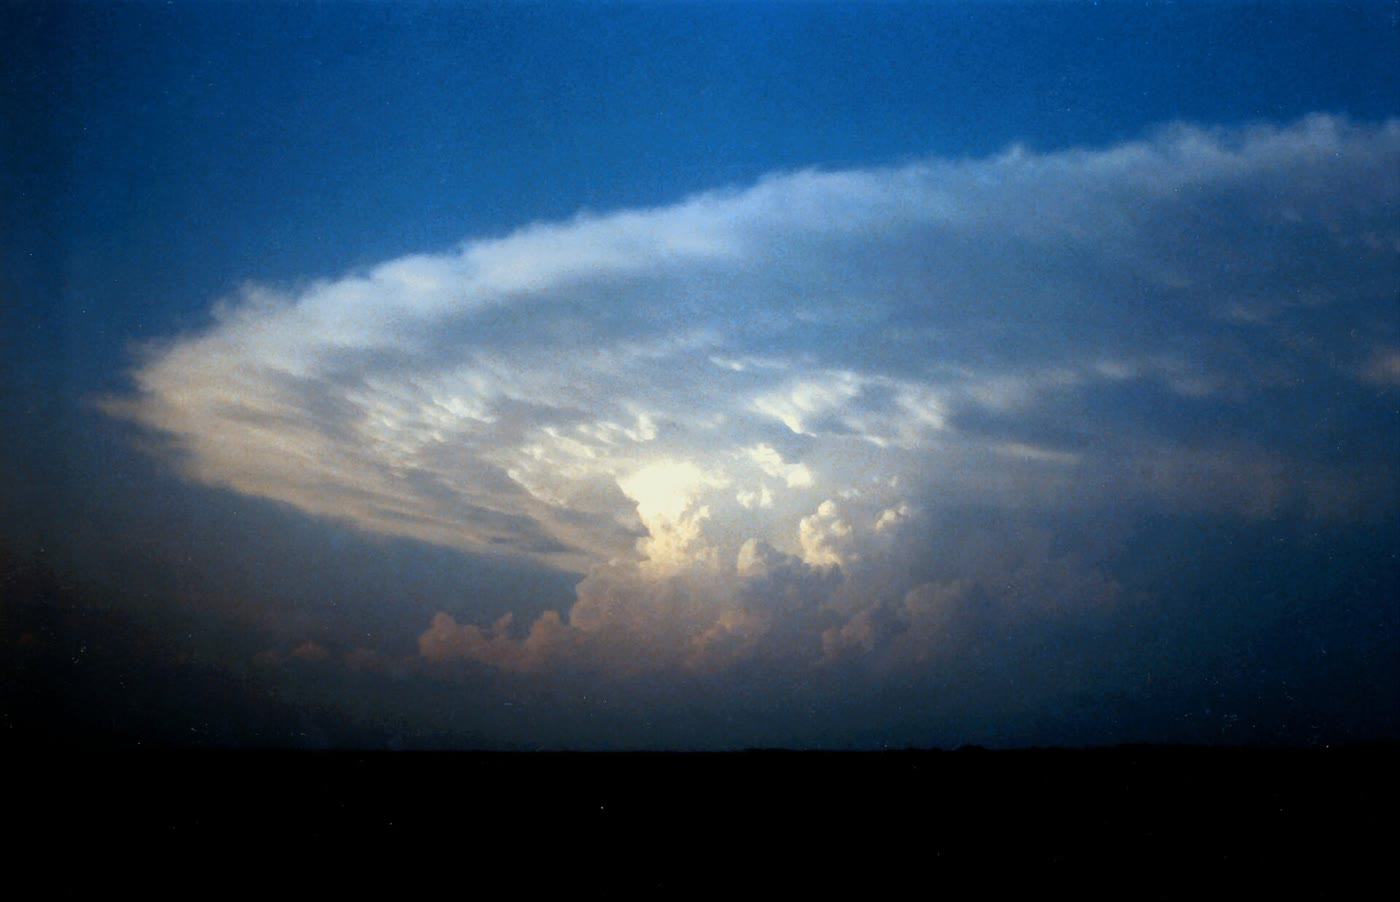
\includegraphics[width=0.6\linewidth]{images/book4/b2-21-supercell-anvil.jpg}
\par\smallskip{\small Een onweersbui boven Nebraska, 20 april 1985: haar opwaartse stroming spreidt zich uit tot
een aambeeld waar ze haar \omterm{def:b2:atmospheric-thermodynamics:parcel-levels}{evenwichtsniveau} bereikt, bij de tropopauze. (Stephen Corfidi,
NOAA/NWS, publiek domein, via Wikimedia Commons.)}
\end{omfigure}
% ledger: nws4:lfc-el

\section{Wolkenmicrofysica}\label{sec:b2:atmospheric-thermodynamics:microphysics}

Een pakketje op zijn LCL is verzadigd boven een vlak wateroppervlak. Een druppel is niet vlak: de
natuurkundeboeken tonen dat een nieuwe fase niet bij evenwicht verschijnt, maar alleen door nucleatie, en de
scheikundeboeken dat de \omterm{def:b2:atmospheric-thermodynamics:moist-air}{dampdruk} boven een gekromd oppervlak groter is dan boven een vlak
(de kelvinvergelijking). Met de constante $A$ van \cref{prop:b2:atmospheric-thermodynamics:kohler}
verderop is een druppel zuiver water van \qty{2}{nm} doorsnede alleen in evenwicht bij de
verzadigingsverhouding $\exp(2.1/2) = 2.9$, een \omterm{def:b2:atmospheric-thermodynamics:microphysics}{oververzadiging} van \qty{190}{\percent}, ver boven de fracties van een
procent waarbij deeltjes worden geactiveerd: druppels ontstaan op deeltjes.

\begin{definition}[Oververzadiging; wolkencondensatiekern]\label{def:b2:atmospheric-thermodynamics:microphysics}
De \emph{oververzadiging}\index{oververzadiging} van lucht is $s = e/e_s - 1$, het overschot van haar
\omterm{def:b2:atmospheric-thermodynamics:moist-air}{dampdruk} boven de verzadigingsdampdruk boven een vlak oppervlak van zuiver water, meestal
in procent gegeven. Een \emph{wolkencondensatiekern}\index{wolkencondensatiekern} (CCN)
is een aerosoldeeltje waarop een wolkendruppel ontstaat bij de kleine oververzadigingen van wolken.
Het is de \emph{condensatiekern}\index{condensatiekern} van de schoolboeken.
\end{definition}
% ledger: nws4:ccn-bergeron, pk07:kohler, morrison20:processes

\begin{proposition}[Köhlerkromme]\label{prop:b2:atmospheric-thermodynamics:kohler}
\index{Köhlerkromme}
Een oplossingsdruppel met diameter $D$, gegroeid op een droog deeltje met diameter $D_d$ en hygroscopiciteit
$\kappa$, is in evenwicht bij de verzadigingsverhouding
\[
  S(D) = \frac{D^3 - D_d^3}{D^3 - D_d^3(1 - \kappa)}\,\exp\Bigl(\frac{A}{D}\Bigr), \qquad
  A = \frac{4\sigma M_w}{R T\rho_w},
\]
met $\sigma$ de oppervlaktespanning en $\rho_w$ de dichtheid van water (aangenomen). De kromme $S(D)$
is de \emph{\omterm{prop:b2:atmospheric-thermodynamics:kohler}{Köhlerkromme}}. Voor $D \gg D_d$ geldt
\[
  s = S - 1 \approx \frac{A}{D} - \frac{\kappa D_d^3}{D^3},
\]
die maximaal is bij de kritieke diameter en \omterm{def:b2:atmospheric-thermodynamics:microphysics}{oververzadiging}
\[
  D_c = \sqrt{\frac{3\kappa D_d^3}{A}}, \qquad s_c = \sqrt{\frac{4A^3}{27\,\kappa D_d^3}} .
\]
\end{proposition}
% ledger: pk07:kohler

\begin{proof}[Bewijs van de benadering]
De exponentiële factor is de kelvinfactor; de breuk is de wateractiviteit, een versie van de wet van
Raoult waarin $\kappa$ meet hoeveel water de opgeloste stof bindt. Voor $D \gg D_d$ en
$A \ll D$ is $\exp(A/D) \approx 1 + A/D$ en is de breuk in eerste orde $1 - \kappa D_d^3/D^3$;
het product is in eerste orde $1 + A/D - \kappa D_d^3/D^3$. De afgeleide
$-A/D^2 + 3\kappa D_d^3/D^4$ gelijk aan nul stellen geeft $D_c^2 = 3\kappa D_d^3/A$, en dan $s_c = A/D_c -
A/(3D_c) = 2A/(3D_c)$, wat de formule is.
\end{proof}

Met $\sigma = \qty{0.072}{J/m^2}$ bij \qty{298.15}{K} is $A = \qty{2.1}{nm}$. Ammoniumsulfaat heeft
$\kappa = 0.61$; natriumchloride is nog hygroscopischer ($\kappa = 1.28$), en atmosferische deeltjes liggen meestal tussen 0.1 en 0.9.
Een droog deeltje ammoniumsulfaat van \qty{50}{nm} heeft $D_c = \qty{0.33}{\micro m}$ en $s_c =
\qty{0.42}{\percent}$; een van \qty{100}{nm} \qty{0.93}{\micro m} en \qty{0.15}{\percent}. De
benadering wijkt minder dan \qty{1}{\percent} af van het exacte maximum.
% ledger: pk07:kohler, pk07:kappa

\begin{omfigure}
\centering
% figdata/bachelor-2/thermo.py part kohler
\begin{tikzpicture}
\begin{semilogxaxis}[width=0.72\linewidth, height=5.6cm, xmin=0.03, xmax=10, ymin=-0.4,
  ymax=1.1, xlabel={druppeldiameter $D$ (\unit{\micro m})}, ylabel={oververzadiging $s$
  (\unit{\percent})}, tick label style={font=\scriptsize}, label style={font=\small},
  log ticks with fixed point, legend style={font=\scriptsize, draw=none, fill=none},
  legend pos=north east, legend cell align=left, unbounded coords=discard]
\addplot[ocBlue, thick, densely dotted] table[x=D_um, y=s30] {figdata/out/bachelor-2-thermo-kohler.dat};
\addlegendentry{$D_d = \qty{30}{nm}$}
\addplot[ocBlue, thick] table[x=D_um, y=s50] {figdata/out/bachelor-2-thermo-kohler.dat};
\addlegendentry{$D_d = \qty{50}{nm}$}
\addplot[ocBlue, thick, dashed] table[x=D_um, y=s100] {figdata/out/bachelor-2-thermo-kohler.dat};
\addlegendentry{$D_d = \qty{100}{nm}$}
\addplot[only marks, mark=*, mark size=1.5pt, black] coordinates {(0.1542,0.914) (0.3309,0.4244)
  (0.9345,0.1499)};
\draw[black!45] (axis cs:0.03,0) -- (axis cs:10,0);
\draw[ocRed, densely dashed] (axis cs:0.03,0.5) -- (axis cs:10,0.5);
\node[font=\scriptsize, ocRed, anchor=north west] at (axis cs:2.2,0.5) {$s = \qty{0.5}{\percent}$};
\end{semilogxaxis}
\end{tikzpicture}
\par\smallskip{\small \omterm{prop:b2:atmospheric-thermodynamics:kohler}{Köhlerkrommen} van deeltjes ammoniumsulfaat ($\kappa = 0.61$) met drie droge
diameters bij \qty{298.15}{K}, met hun kritieke punten (stippen). In lucht met \qty{0.5}{\percent}
\omterm{def:b2:atmospheric-thermodynamics:microphysics}{oververzadiging} groeien de deeltjes van \qty{50}{nm} en \qty{100}{nm} onbeperkt; het deeltje van
\qty{30}{nm} blijft een neveldruppel.}
\end{omfigure}
% ledger: pk07:kohler, pk07:kappa

De kromme verdeelt de deeltjes. Onder haar top is een druppel in stabiel evenwicht: als hij groeit,
is de lucht niet langer oververzadigd genoeg voor hem en krimpt hij terug; zulke neveldruppels zwellen
en krimpen met de vochtigheid. Zodra de \omterm{def:b2:atmospheric-thermodynamics:microphysics}{oververzadiging} van de lucht $s_c$ overschrijdt, is de druppel
\emph{geactiveerd}: voorbij de top heeft hij steeds minder \omterm{def:b2:atmospheric-thermodynamics:microphysics}{oververzadiging} nodig naarmate hij groeit, en hij groeit
zolang er damp is. Een stijgend pakketje koelt af, zijn \omterm{def:b2:atmospheric-thermodynamics:microphysics}{oververzadiging} klimt, en de grootste
en best oplosbare deeltjes worden het eerst geactiveerd; de druppels die ze vormen, nemen dan de damp op en
begrenzen de \omterm{def:b2:atmospheric-thermodynamics:microphysics}{oververzadiging}. Boven afgelegen oceanen zijn er ongeveer 110 CCN per kubieke centimeter actief
bij \qty{0.4}{\percent}, boven afgelegen continenten bijna twee keer zoveel, en in vervuilde lucht ongeveer
tien keer meer. Hetzelfde water verdeeld over meer druppels maakt ze kleiner.
% ledger: andreae09:ccn, morrison20:processes

\begin{remark}[Waarom condensatie alleen geen regen maakt]\label{rem:b2:atmospheric-thermodynamics:growth}
Een druppel groeit door de diffusie van damp naar hem toe. De flux door een bol rond een druppel
met straal $r$ is $4\pi r D_v\,\Delta\rho_v$, met $D_v$ de diffusiecoëfficiënt van damp en
$\Delta\rho_v$ het overschot aan dampdichtheid ver weg, dus zijn massa $\tfrac43\pi r^3\rho_w$ groeit
met een snelheid evenredig met $r$: $r\,\mathrm{d}r/\mathrm{d}t$ is constant en $r^2$ groeit lineair in
de tijd. Grote druppels groeien trager dan kleine, en een populatie die alleen door condensatie
groeit, wordt smaller, niet breder. Regendruppels ontstaan wanneer druppels van verschillende grootte, die met
verschillende snelheden vallen, botsen en samensmelten.
\end{remark}
% ledger: morrison20:processes

Boven het niveau van \qty{0}{\celsius} bestaat een wolk uit onderkoelde druppels tot ijskiemen
ijskristallen doen ontstaan. Dan werkt het verschil uit het rechterpaneel van de
verzadigingsfiguur: lucht die boven de druppels verzadigd is, is \qty{10}{\percent} oververzadigd boven
ijs bij \qty{-10}{\celsius}, tientallen keren de \omterm{def:b2:atmospheric-thermodynamics:microphysics}{oververzadigingen} waarbij de druppels werden geactiveerd.
De kristallen groeien door depositie ten koste van de druppels, die verdampen (het Bergeron%
proces, het ijskristalproces van de schoolboeken), en ze vangen druppels in die op hen
bevriezen (aanvriezing).
% ledger: nws4:ccn-bergeron, morrison20:processes, iapws4:sublimation

\begin{omfigure}
\centering
\begin{tikzpicture}[font=\scriptsize, box/.style={draw=black!60, rounded corners=2pt,
  align=center, minimum height=0.95cm, text width=2.1cm, fill=#1}, box/.default=white,
  >=Stealth]
\node[anchor=west, black!60] at (-1.15,0.8) {warme processen};
\node[box=black!6] (ccn) at (0,0) {aerosoldeeltje\\(CCN)};
\node[box=ocBlue!8] (haze) at (4.2,0) {neveldruppel\\$s < s_c$};
\node[box=ocBlue!15] (act) at (8.4,0) {geactiveerde druppel\\$s > s_c$};
\node[box=ocBlue!25] (rain) at (12.6,0) {regendruppel};
\draw[->] (ccn) -- node[above] {vochtigheid} (haze);
\draw[->] (haze) -- node[above] {stijging} (act);
\draw[->] (act) -- node[above, align=center] {botsing,\\samen-\\smelting} (rain);
\node[anchor=west, black!60] at (-1.15,-3.4) {ijsprocessen};
\node[box=black!6] (inp) at (0,-2.6) {ijskiem};
\node[box=omMeth!10] (ice) at (4.2,-2.6) {ijskristal\\onder \qty{0}{\celsius}};
\node[box=omMeth!20] (snow) at (8.4,-2.6) {sneeuw, korrelhagel};
\node[box=ocBlue!25] (rain2) at (12.6,-2.6) {regen};
\draw[->] (inp) -- (ice);
\draw[->] (ice) -- node[above, align=center] {depositie,\\aanvriezing} (snow);
\draw[->] (snow) -- node[above] {smelten} (rain2);
\draw[->, omMeth!60!black, dashed] (act.south) -- node[pos=0.45, right=4pt, align=left,
  omMeth!60!black] {damp van de\\verdampende druppels} (ice.north);
\end{tikzpicture}
\par\smallskip{\small De twee wegen van damp naar neerslag: activering en groei van
druppels, daarna botsing en samensmelting (boven); ijskristallen die groeien ten koste van
onderkoelde druppels, aanvriezen en smelten wanneer ze in warmere lucht vallen (onder).}
\end{omfigure}
% ledger: morrison20:processes, nws4:ccn-bergeron

\begin{inthefield}[Een lancering in de ochtend]
\begin{minipage}[t]{0.54\linewidth}\vspace{0pt}
Op elk hoogteweerstation maakt de technicus de ballon en de radiosonde klaar in het uur
vóór 00 en 12 UTC, de tijdstippen waarop meer dan achthonderd stations van de wereld
samen waarnemen. Het instrument, van 60 tot \qty{80}{g}, hangt onder de ballon en meldt elke seconde de druk,
de temperatuur, de vochtigheid en zijn satellietpositie. De ballon stijgt ongeveer
\qty{300}{m} per minuut, twee uur of langer, tot voorbij \qty{35}{km} voordat hij barst, en kan
meer dan \qty{300}{km} afdrijven. Weervoorspellers zetten het profiel uit op een scheve-T-diagram, en op
dagen waarop zwaar weer wordt verwacht, laten sommige stations extra ballonnen op.
\end{minipage}\hfill
\begin{minipage}[t]{0.42\linewidth}\vspace{0pt}
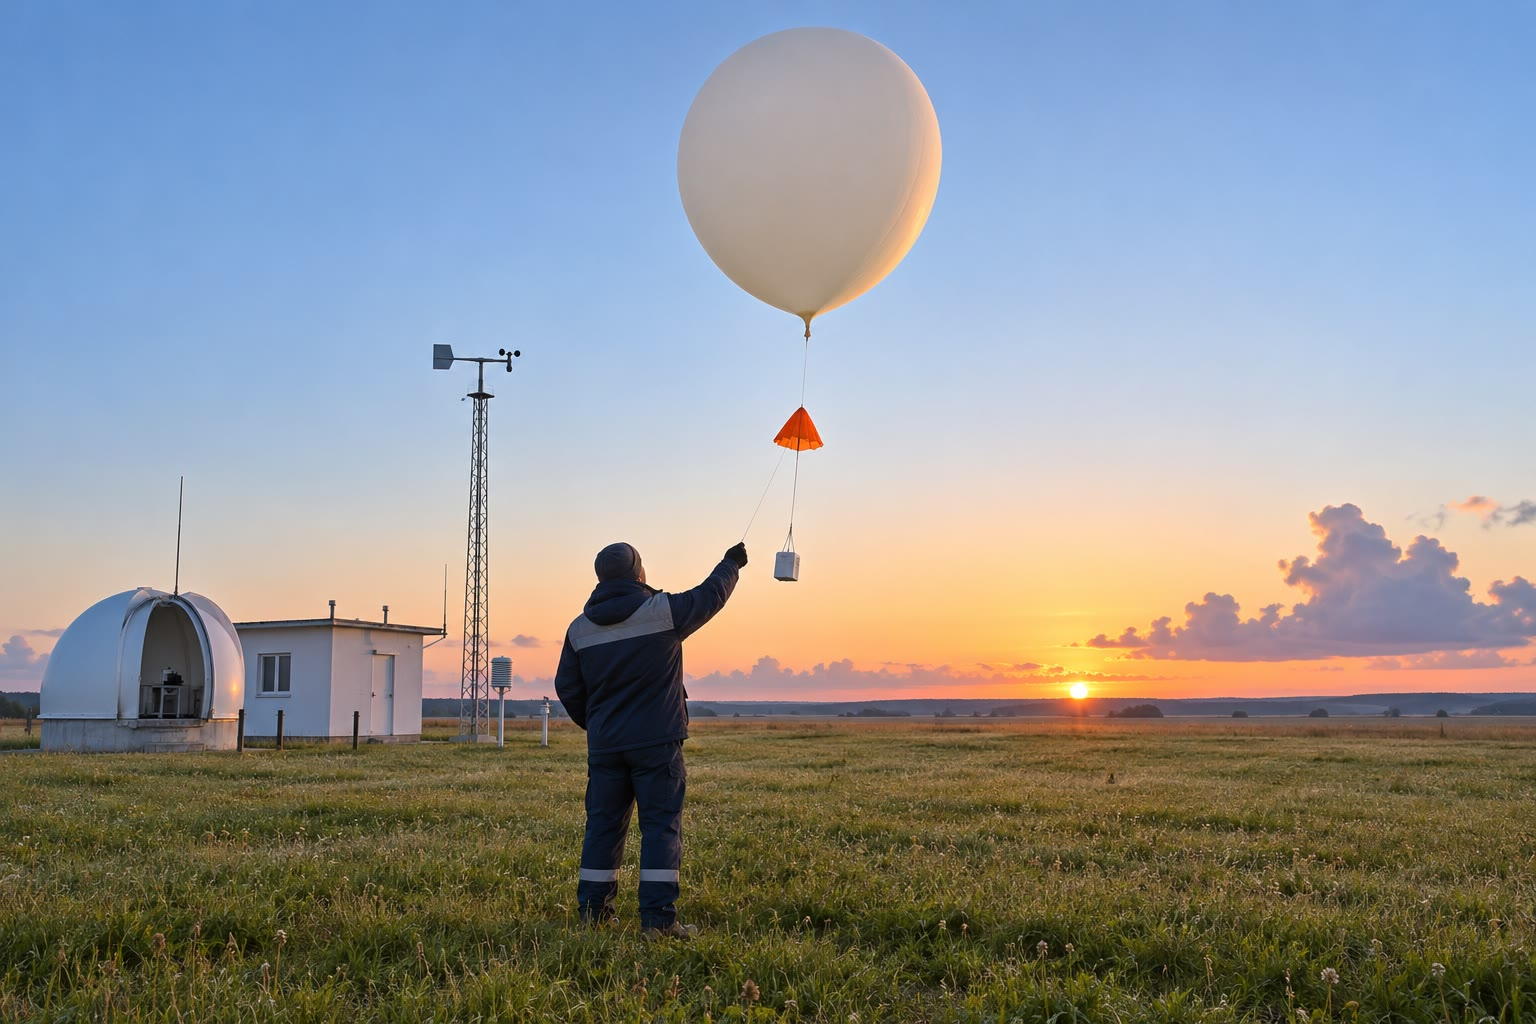
\includegraphics[width=\linewidth]{images/book4/ai/b2-radiosonde-launch.jpg}

{\scriptsize Een radiosonde die bij dageraad van een weerstation wordt losgelaten (door AI gegenereerde
illustratie).}
\end{minipage}
% ledger: nws:radiosonde, nws4:upperair
\end{inthefield}

\section*{Oefeningen}\label{sec:b2:atmospheric-thermodynamics:exercises}

Gegevens voor de oefeningen, tenzij anders vermeld: $e_s(T) = \qty{6.117}{hPa} \times
\exp[\qty{5419}{K} \times (1/\qty{273.16}{K} - 1/T)]$; $\varepsilon = 0.622$, $R_d =
\qty{287.0}{J.kg^{-1}.K^{-1}}$, $R_v = \qty{461.5}{J.kg^{-1}.K^{-1}}$, $c_p =
\qty{1004.5}{J.kg^{-1}.K^{-1}}$, $L = \qty{2.501e6}{J/kg}$, $g = \qty{9.81}{m.s^{-2}}$,
$\Gamma_d = \qty{9.8}{K/km}$.
% ledger: nist4:water-sat, iapws4:sublimation, const:R, earth:Mmol, nist4:water-mw, nasa:grc-gamma

\begin{exercise}[$\star$]\label{exo:b2:atmospheric-thermodynamics:1}
Bij \qty{850}{hPa} is de temperatuur \qty{10.0}{\celsius} en het dauwpunt \qty{5.0}{\celsius}.
(a) Bepaal de \omterm{def:b2:atmospheric-thermodynamics:moist-air}{dampdruk} en de verzadigingsdampdruk. (b) Bepaal de relatieve vochtigheid.
(c) Bepaal de \omterm{def:b2:atmospheric-thermodynamics:moist-air}{mengverhouding} en de \omterm{def:b2:atmospheric-thermodynamics:moist-air}{specifieke vochtigheid}, in gram per kilogram.
\end{exercise}

\begin{exercise}[$\star$]\label{exo:b2:atmospheric-thermodynamics:2}
(a) Met hoeveel procent per kelvin stijgt $e_s$ bij \qty{0}{\celsius}, \qty{20}{\celsius} en
\qty{30}{\celsius}? (b) Bereken $e_s$ bij \qty{20}{\celsius} en bij \qty{25}{\celsius}, en hun
verhouding; vergelijk met $1.063^5$. (c) De gemeten waarde bij \qty{20}{\celsius} is
\qty{23.39}{hPa}. Hoeveel wijkt de formule af, en in welke richting? Waarom?
\end{exercise}
% ledger: nist4:water-sat

\begin{exercise}[$\star$]\label{exo:b2:atmospheric-thermodynamics:3}
Om twaalf uur 's middags is de oppervlaktelucht \qty{30}{\celsius} met een dauwpunt van \qty{14}{\celsius}. (a) Op
welke hoogte boven de grond ontstaan de basissen van cumuluswolken? (b) Wat is daar de temperatuur van een pakketje,
volgens de droge adiabaat? (c) Wat is daar zijn dauwpunt, met $\Gamma_{\text{dauw}} =
\qty{1.8}{K/km}$? Becommentarieer. (d) Later warmt de lucht op tot \qty{33}{\celsius}, met ongewijzigd
dauwpunt. Waar liggen de wolkenbases nu?
\end{exercise}

\begin{exercise}[$\star$]\label{exo:b2:atmospheric-thermodynamics:4}
Lees het scheve-T-diagram van de sondering van Norman af. (a) Tot welke druk is de lucht bij de
grond verzadigd, of bijna? (b) Waar ligt de inversie, en hoe is ze te zien? (c) Lees het
LCL, het LFC en het EL van het oppervlaktepakketje af. (d) Hoe verhouden het dauwpunt en de temperatuur
zich net boven de inversie, en wat zegt dat over deze lucht?
\end{exercise}
% ledger: data:b4-sounding

\begin{exercise}[$\star\star$]\label{exo:b2:atmospheric-thermodynamics:5}
Tropische lucht bij \qty{1000}{hPa} heeft $T = \qty{30.0}{\celsius}$ en $r = \qty{20}{g/kg}$. (a) Bepaal
haar \omterm{def:b2:atmospheric-thermodynamics:virtual}{virtuele temperatuur} exact en met de benadering $T(1 + 0.61\,r)$. (b) Bepaal de dichtheden
van deze lucht en van droge lucht bij dezelfde temperatuur en druk. (c) Hoeveel zou droge lucht
moeten worden opgewarmd om even licht te zijn? (d) Waarom is dit van belang voor convectie boven warme zeeën?
\end{exercise}

\begin{exercise}[$\star\star$]\label{exo:b2:atmospheric-thermodynamics:6}
Gebruik \cref{prop:b2:atmospheric-thermodynamics:gamma-s} bij \qty{1000}{hPa}, met $r_s$ uit
\cref{prop:b2:atmospheric-thermodynamics:humidity}. (a) Bereken $r_s$ en $\Gamma_s$ bij
\qty{0}{\celsius}, \qty{20}{\celsius} en \qty{30}{\celsius}. (b) Hoeveel warmer dan een droog
pakketje is een verzadigd pakketje bij \qty{20}{\celsius} nadat het \qty{1}{km} is gestegen, als zijn gradiënt
gelijk blijft? (c) Waarom wordt het verschil hogerop kleiner?
\end{exercise}

\begin{exercise}[$\star\star$]\label{exo:b2:atmospheric-thermodynamics:7}
Het oppervlaktepakketje van Norman ($p = \qty{971.1}{hPa}$, $T = \qty{19.0}{\celsius}$, $T_d =
\qty{18.5}{\celsius}$) heeft zijn LCL bij \qty{18.35}{\celsius}. (a) Bereken zijn \omterm{def:b2:atmospheric-thermodynamics:moist-air}{mengverhouding}, zijn
potentiële temperatuur en zijn \omterm{def:b2:atmospheric-thermodynamics:theta-e}{equivalent-potentiële temperatuur}. (b) Opgetild is het
\qty{-8.9}{\celsius} bij \qty{500}{hPa}, verzadigd. Bereken daar zijn $\theta$ en $\theta_e$.
(c) Welke van de twee blijft behouden?
\end{exercise}
% ledger: data:b4-sounding

\begin{exercise}[$\star\star$]\label{exo:b2:atmospheric-thermodynamics:8}
Een pakketje is \qty{4}{K} warmer dan zijn omgeving tussen \qty{700}{hPa}, zijn LFC, en
\qty{300}{hPa}, zijn EL; verwaarloos de correctie voor de \omterm{def:b2:atmospheric-thermodynamics:virtual}{virtuele temperatuur}. (a) Bereken zijn CAPE. (b)
Bereken $w_{\max}$. (c) In welke klasse valt de CAPE? (d) Welke vorm heeft de positieve oppervlakte op een
scheve-T-diagram, en waarom is haar oppervlakte wat werd berekend?
\end{exercise}
% ledger: hgx:cape

\begin{exercise}[$\star\star$]\label{exo:b2:atmospheric-thermodynamics:9}
Neem $A = \qty{2.1}{nm}$ en ammoniumsulfaat, $\kappa = 0.61$. (a) Bepaal de kritieke diameter
en \omterm{def:b2:atmospheric-thermodynamics:microphysics}{oververzadiging} van een droog deeltje van \qty{80}{nm}. (b) Wat is het kleinste droge deeltje dat
wordt geactiveerd in lucht met \qty{0.3}{\percent} \omterm{def:b2:atmospheric-thermodynamics:microphysics}{oververzadiging}? Bij \qty{0.1}{\percent}? (c) Een opwaartse stroming
verhoogt de \omterm{def:b2:atmospheric-thermodynamics:microphysics}{oververzadiging} van \qty{0.1}{\percent} tot \qty{0.3}{\percent}: wat gebeurt er met het
aantal druppels, en met hun grootte bij hetzelfde vloeibare water?
\end{exercise}
% ledger: pk07:kappa, pk07:kohler

\begin{exercise}[$\star\star\star$]\label{exo:b2:atmospheric-thermodynamics:10}
Het oppervlaktepakketje van Norman had een CIN van ongeveer \qty{-130}{J/kg} met de \omterm{def:b2:atmospheric-thermodynamics:virtual}{virtuele temperatuur}.
(a) Met welke verticale snelheid zou het de grond moeten verlaten om zijn LFC op eigen
impuls te bereiken? (b) De top van de inversie ligt bij \qty{889.1}{hPa} en \qty{20.5}{\celsius}. Tot welke
temperatuur moet de oppervlaktelucht bij \qty{971.1}{hPa} opwarmen opdat een droogadiabatisch
opgetild pakketje niet kouder is dan de top van de inversie? (c) Als haar dauwpunt op
\qty{18.5}{\celsius} bleef, waar zou haar wolkenbasis liggen? (d) Noem twee manieren waarop de atmosfeer
zo'n deksel zonder de zon verwijdert.
\end{exercise}
% ledger: data:b4-sounding, nws4:cin

\begin{exercise}[$\star\star\star$]\label{exo:b2:atmospheric-thermodynamics:11}
(a) Toon met \cref{prop:b2:atmospheric-thermodynamics:gamma-s} aan dat $\Gamma_s \to \Gamma_d$
als $r_s \to 0$. (b) Toon aan dat, wanneer $Lr_s/(R_dT) \gg 1$, $\Gamma_s \to gR_vT/(LR_d)$, en
bereken dit bij \qty{303}{K}. (c) Vergelijk met $\Gamma_{\text{dauw}}$ van
\cref{prop:b2:atmospheric-thermodynamics:lcl} wanneer $T_d = T$, en verklaar waarom de twee limieten
samenvallen. (d) Wordt de limiet van (b) in de atmosfeer bereikt? Gebruik de waarde $\Gamma_s =
\qty{3.4}{K/km}$ bij \qty{30}{\celsius} en \qty{1000}{hPa}.
\end{exercise}

\begin{exercise}[$\star\star\star$]\label{exo:b2:atmospheric-thermodynamics:12}
Boven onderkoeld water en boven ijs zijn de verzadigingsdampdrukken 2.868 en
\qty{2.599}{hPa} bij \qty{-10}{\celsius}, 1.257 en \qty{1.032}{hPa} bij \qty{-20}{\celsius}.
(a) Bepaal de \omterm{def:b2:atmospheric-thermodynamics:microphysics}{oververzadiging} ten opzichte van ijs van lucht die boven water verzadigd is, bij beide temperaturen. (b)
Vergelijk met de \omterm{def:b2:atmospheric-thermodynamics:microphysics}{oververzadigingen} waarbij druppels worden geactiveerd. (c) Verklaar waarom een wolk van
onderkoelde druppels die enkele ijskristallen ontvangt, in ijs overgaat. (d) Waarom is het effect
zwakker bij \qty{0}{\celsius}?
\end{exercise}
% ledger: iapws4:sublimation, su26:svp, nws4:ccn-bergeron

\begin{problem}[{Weekendprobleem --- De ochtendsondering lezen}]\label{pb:b2:atmospheric-thermodynamics:1}
De tabel geeft de sondering van 12 UTC in Norman, Oklahoma, op 16 april 2026, op de niveaus die
hier worden gebruikt: druk, hoogte boven zeeniveau, temperatuur, dauwpunt, en de temperatuur van het
oppervlaktepakketje, opgetild zoals in \cref{met:b2:atmospheric-thermodynamics:lift} en berekend door
\cref{prop:b2:atmospheric-thermodynamics:gamma-s} in kleine stappen te integreren. De sondering
meldt de tropopauze bij \qty{235.3}{hPa} en \qty{10954}{m}. Gebruik de gegevens van de oefeningen en
de temperaturen (niet de \omterm{def:b2:atmospheric-thermodynamics:virtual}{virtuele temperaturen}), tenzij anders aangegeven.

\begin{center}
\small
\begin{tabular}{rrrrr}
\hline
$p$ (\unit{hPa}) & $z$ (\unit{m}) & $T$ (\unit{\celsius}) & $T_d$ (\unit{\celsius}) &
$T_{\text{pakketje}}$ (\unit{\celsius}) \\
\hline
971.1 & 345 & 19.0 & 18.5 & 19.0 \\
925.0 & 763 & 17.3 & 17.3 & 16.9 \\
907.7 & 924 & 16.4 & 16.4 & 16.2 \\
889.1 & 1102 & 20.5 & 9.5 & 15.4 \\
850.0 & 1489 & 18.6 & $-1.8$ & 13.7 \\
700.0 & 3110 & 4.5 & $-12.2$ & 6.1 \\
500.0 & 5725 & $-18.4$ & $-36.6$ & $-8.9$ \\
400.0 & 7357 & $-30.4$ & $-55.6$ & $-20.4$ \\
300.0 & 9349 & $-42.7$ & $-66.3$ & $-37.1$ \\
250.0 & 10560 & $-49.8$ & $-69.8$ & $-48.3$ \\
200.0 & 12006 & $-52.3$ & $-78.3$ & $-61.8$ \\
\hline
\end{tabular}
\end{center}

\medskip\noindent\textbf{Deel I --- De lucht bij de grond.}
\begin{enumerate}
  \item Bepaal de \omterm{def:b2:atmospheric-thermodynamics:moist-air}{dampdruk} van de oppervlaktelucht, op één decimaal.
  \item Bepaal haar \omterm{def:b2:atmospheric-thermodynamics:moist-air}{mengverhouding}, op één decimaal.
  \item Bepaal haar \omterm{def:b2:atmospheric-thermodynamics:moist-air}{specifieke vochtigheid}.
  \item Bepaal haar relatieve vochtigheid.
  \item Hoeveel is haar \omterm{def:b2:atmospheric-thermodynamics:virtual}{virtuele temperatuur} hoger dan haar temperatuur?
  \item Bepaal de hoogte van haar LCL boven de grond met de regel van \qty{125}{m}, en de druk
        daar (neem voor de laag een gemiddelde \omterm{def:b2:atmospheric-thermodynamics:virtual}{virtuele temperatuur} van \qty{294.7}{K}).
  \item Bepaal haar potentiële temperatuur.
\end{enumerate}

\medskip\noindent\textbf{Deel II --- Het deksel en de lagen erboven.}
\begin{enumerate}[resume]
  \item Is het pakketje bij \qty{925}{hPa} warmer of kouder dan zijn omgeving, en hoeveel?
  \item Bepaal de gradiënt tussen 907.7 en \qty{889.1}{hPa}. Wat voor laag is dit?
  \item Hoeveel is het pakketje bij \qty{889.1}{hPa} kouder dan zijn omgeving?
  \item Bepaal de relatieve vochtigheid bij \qty{850}{hPa}. Waar zou zulke lucht vandaan kunnen komen?
  \item Bepaal de gemiddelde gradiënt tussen 850 en \qty{500}{hPa} en classificeer de laag.
  \item Bepaal de lifted index en zijn klasse.
\end{enumerate}

\medskip\noindent\textbf{Deel III --- De energie.}
\begin{enumerate}[resume]
  \item Bereken het overschot $\Delta T = T_{\text{pakketje}} - T$ op elk niveau van de tabel.
  \item Bepaal het LFC door $\Delta T$ lineair in $\ln p$ te interpoleren, op de hectopascal nauwkeurig,
        en zijn hoogte door $z$ op dezelfde manier te interpoleren.
  \item Bepaal het EL en zijn hoogte op dezelfde manier. Vergelijk met de tropopauze.
  \item Bereken de CAPE met de trapeziumregel in $\ln p$, van het LFC tot het EL via de
        niveaus van de tabel.
  \item In welke klasse valt ze?
  \item Bereken de CIN op dezelfde manier, van de grond tot het LFC.
  \item Een berekening op een rooster van \qty{1}{hPa} geeft een CAPE van \qty{2100}{J/kg} met de
        temperaturen en \qty{2230}{J/kg} met de \omterm{def:b2:atmospheric-thermodynamics:virtual}{virtuele temperaturen}. Waarom verschillen de drie
        waarden?
\end{enumerate}

\medskip\noindent\textbf{Deel IV --- De onweersbui die de lucht kon voeden.}
\begin{enumerate}[resume]
  \item Welke verticale snelheid geeft de pakketjestheorie met de CAPE van vraag 17?
  \item Hoe lang zou de lucht, met overal de helft van die snelheid, erover doen om van het LFC naar het EL te stijgen?
  \item Noem twee effecten die een echte opwaartse stroming trager maken.
  \item Samengevat: welke snelheid van de opwaartse stroming voorspelt de pakketjestheorie voor een onweersbui die door de
        oppervlaktelucht van deze ochtend wordt gevoed?
\end{enumerate}
\end{problem}
% ledger: data:b4-sounding, hgx:cape, nws4:lifted-index, nws4:cape
